\documentclass[10pt,a4paper]{article}

\usepackage[margin=1in]{geometry}
\usepackage[UKenglish]{babel}
\usepackage{enumitem}
\usepackage{calc}
\usepackage{fancyhdr}
\usepackage{graphicx}
\usepackage{multirow}
\usepackage[table]{xcolor}
\usepackage{float}
\usepackage{longtable}
\usepackage{parskip}
\usepackage{soul}
\usepackage{ifthen}
\usepackage[compact]{titlesec}
\usepackage[justification=centering]{caption}
\usepackage{subcaption}


\definecolor{reqColor}{RGB}{80,80,120}

%%Tables
\newcommand{\tableformat}[4]{
\begin{table}[H]
\centering
  \rowcolors{2}{gray!10} {white}
\begin{tabular}{#1}
  \hline
  \rowcolor[gray]{0.9} #2
\end{tabular}
\caption{#3}
\label{#4}
\end{table}}

\pagestyle{fancy}
\lhead{T Davies, A Fahie, A Fairbairn, A Free, J Mansfield, R Tucker, M 
Walker}
\chead{}
\rhead{GPIG-C}
\cfoot{\vspace{-0.6cm} \thepage}

\setlist{nolistsep} % Reduces lots of white space around lists

\renewcommand{\headrulewidth}{0.4pt} % Add rules below header
\renewcommand*{\thefootnote}{\fnsymbol{footnote}}

\newcommand{\conreq}[1]{\textcolor{reqColor}{\textbf{CR.#1}}}
\newcommand{\fr}[1]{\textcolor{reqColor}{\textbf{FR.#1}}}
\newcommand{\ed}[1]{\textcolor{reqColor}{\textbf{ED.#1}}}
\newcommand{\nfr}[1]{\textcolor{reqColor}{\textbf{NFR.#1}}}
\newcommand{\qas}[1]{\textcolor{reqColor}{\textbf{QAS.#1}}}
		
		


%%Scenarios
\newenvironment{scenario}[1]{
\newcommand{\source}[1]{\item[Source of Stimulus:] ##1}
\newcommand{\stimulus}[1]{\item[Stimulus:] ##1}
\newcommand{\artifact}[1]{\item[Artifact:] ##1}
\newcommand{\environment}[1]{\item[Environment:] ##1}
\newcommand{\response}[1]{\item[Response:] ##1}
\newcommand{\measure}[1]{\item[Response Measure:] ##1}
\newcommand{\rationale}[1]{\item[Scenario Rationale:] ##1}
\newcommand{\quality}[1]{\item[Quality:] ##1}
		\begin{description} [noitemsep]	
		\item[Scenario ID:] \qas{#1}
		}{\end{description} \vspace*{0.3cm}
		}

%%Requirements
\newenvironment{requirements}{
\newcommand{\requirement}[3]{\item[\fr{##1}] ##2
							\ifx&##3&
							%nothing
							\else
								\begin{description}
									##3
								\end{description}							
							\fi
							}
		\begin{description}[noitemsep, leftmargin=1.3cm]	
		}{\end{description} \vspace*{0.3cm}
		}
		
\begin{document}
\begin{center}
{\vspace*{-0.5cm}
\Huge GPIG-C Final Report}
\vspace*{0.2cm}

Word count: @WORD_COUNT@
 (\textit{using TeXCount})
\vspace*{0.1cm}

Wednesday, 21st May 2014
\end{center}
\vspace*{0.4cm}
\hrule
\vspace*{0.4cm}

%-------------------------------------------------------------%
%----------------------INTRODUCTION -------------------%
%-------------------------------------------------------------%
\section{Introduction}
\label{sec:intro}
This report details the design and development of a HUMS, concentrating on progress and changes made since the interim report. In this document the systems requirements are further refined, building on the feedback from the previous report, including a set of external dependencies. The system's architecture is then considered, in order to determine how the system will meet its requirements and what design decisions must be made. This includes examining the quality attributes associated with the system and the related scenarios, as well as tactics and patterns which can be used to achieve these qualities. The desired HUMS architecture is then presented using a number of system views deemed to be important. Having determined the architecture of the system, the risks associated with this design and the project as a whole are discussed, and the risk reduction tactics used to mitigate them are also discussed.

The development of the prototype HUMS, demonstrating some of the important features in the design, is then described, followed by a set of evaluations used to determine the achieved quality and functionality of the system. The project is then concluded, and the team reflects on their decisions throughout the project.

%-------------------------------------------------------------%
%--------------------------GLOSSARY ---------------------%
%-------------------------------------------------------------%
\section{Glossary}
\label{sec:glossary}
\hl{TODO: Possibly update this}
\begin{description}%[leftmargin=!,labelwidth=\widthof{\bfseries Data output clientxx},noitemsep]
	\item[The HUMS/System] The health and usage monitoring system being developed
	\item[(HUMS) Instance] A particular deployment of the System
	\vspace{0.15cm}
	\item[Customer] Thales, the organisation that has commissioned the System
	\item[Consumer] An organisation that makes use of the System
	\item[Consumer System] The system that a Consumer wishes to monitor
	\item[(End) User] An individual that uses the System within a Consumer organisation
	\vspace{0.15cm}
	\item[Client] Computer hardware or software that interfaces with an Instance
	\item[Input Interface] The interface through which data is supplied to an Instance
	\item[Data Emitter] A Client that provides data to an Instance through the Input Interface
	\item[Output Interface] The interfaces through which reports and notifications are dispatched
	\item[Data Output Client] A Client that receives data from an Instance through Output Interfaces
	\item[Admin Centre] \hl{TODO}
	\item[(HUMS) Core] \hl{TODO}
	\vspace{0.15cm}
	\item[Event] A trend in data identified by analysis
	\item[Notification] A message dispatched by the System when an Event is fired
	\item[Report] A message produced by the System at the request of a User
	\vspace{0.14cm}
	\item[Sensor] A source of data to be monitored by the System
	\item[Sensor ID] A unique identifier denoting a particular Sensor
	\item[System ID] A unique identifier denoting a group of Sensors
\end{description}

%-------------------------------------------------------------%
%-------------------REQUIREMENTS----------------------%
%-------------------------------------------------------------%
\section{Requirements Refinement}
\label{sec:requirements}
After feedback from the initial and interim reports, the HUMS requirements have been updated. This included modifying existing requirements and adding additional requirements and refinements. It also included removing the constraint requirements, which were deemed unnecessary by the module leader, and instead identifying the external dependencies of the system.

\subsection{Functional Requirements}
\label{sec:functional_requirements}
\hl{write about changes -- currently they are unchanged} 

\begin{requirements}
\requirement{1}{Data Emitters shall be able to push correctly structured data to the HUMS.}{
	\requirement{1.1}{The HUMS shall provide an API for data input (the Input Interface).}{
		\requirement{1.1.1}{The Input Interface shall require a System ID that uniquely identifies the Consumer System.}{}
		\requirement{1.1.2}{The Input Interface shall require input data to be timestamped.}{}
		\requirement{1.1.3}{The Input Interface shall allow Data Emitters to send Sensor IDs and their values to the HUMS, to be made available to an analysis engine.}{}
	}
	\requirement{1.2}{A Data Emitter for extracting data from the given test application shall be provided.}{}
}
\requirement{2}{The HUMS shall allocate a timestamp to new data.}{
	\requirement{2.1}{Data shall be timestamped before it reaches the HUMS Input Interface.}{}
	\requirement{2.2}{Timestamps shall be stored alongside the input data.}{}
}
\requirement{3}{The HUMS shall store correctly structured data.}{
	\requirement{3.1}{The HUMS shall use a database abstraction layer, allowing the Consumer to select their datastore technology.}{}
}
\requirement{4}{The HUMS shall store End User configuration files.}{
	\requirement{4.1}{The HUMS shall allow authorised Users to modify configuration files.}{}
	\requirement{4.2}{The HUMS shall allow the User to define a storage limit.}{}
	\requirement{4.3}{The HUMS shall allow the User to set an expiry time on stored data.}{}
	\requirement{4.4}{The HUMS shall allow the User to define that, upon reaching their defined data storage quota, new data is no longer stored.}{}
	\requirement{4.5}{The HUMS shall allow the User to define that, upon reaching their defined data storage limit, old data is removed to make room for the new data.}{}
}
\requirement{5}{The HUMS shall dispatch a Notification when the Consumer's storage limit is reached.}{}
\requirement{6}{The HUMS must store no more data records than the Consumer-defined storage quota.}{}
\requirement{7}{Events shall be triggered in response to data matching analysis rules specified by a User.}{
	\requirement{7.1}{The HUMS shall allow the User to specify which analysis rules will produce Events.}{}
	\requirement{7.2}{The HUMS shall allow the User to define their own Events.}{}
	\requirement{7.3}{The HUMS shall provide an API, allowing analysis engines to fetch stored data.}{}
	\requirement{7.4}{Events shall be identified by analysis engines.}{}
	\requirement{7.5}{The HUMS shall provide a simple analysis engine in the form of a rules engine.}{}
}
\requirement{8}{After dispatching a Notification for an Event of a particular type, no more Notifications for an Event of that type will be sent during a User-specified cool down period.}{
	\requirement{8.1}{The HUMS shall allow the User to specify a cool down period for particular Events.}{}
}
\requirement{9}{The HUMS shall identify an Event when a specified analysis rule is matched.}{}
\requirement{10}{The HUMS must interface with Report engines, allowing them to pull Reports.}{}
\requirement{11}{The System shall allow for Notifications to be fed back to the Consumer System to change
the way in which data is sensed.}{}
\end{requirements}

\subsection{Non-Functional Requirements}
\label{sec:nonfunctional_requirements}
\hl{write about changes -- currently they are unchanged} 

\begin{requirements}
\requirement{1}{The HUMS shall undergo hardware modifications without loss of previously stored data.}{}
\requirement{2}{Users shall be provided with documentation detailing how to use the HUMS.}{}
\requirement{3}{The HUMS must be accessible to End Users regardless of their geographic location.}{}
\requirement{4}{The HUMS shall only accept data from a Client of the Input Interface providing valid credentials.}{}
\requirement{5}{The HUMS shall allow data to be stored according to the relevant industry security standards.}{}
\requirement{6}{The HUMS shall be tested to ensure all requirements are met before deployment.}{
	\requirement{6.1}{The HUMS shall be tested using unit testing.}{}
	\requirement{6.2}{The HUMS shall be tested using integration testing.}{}
	\requirement{6.3}{The HUMS shall be tested using system testing.}{}
	\requirement{6.4}{The HUMS shall be tested using inspection.}{}
	\requirement{6.5}{The HUMS shall be tested using acceptance testing.}{}
}
\requirement{7}{The Customer will complete acceptance testing before the System is deployed.}{}
\requirement{8}{The System must be able to support at least 5 Clients of the Output Interface per HUMS Instance.}{}
\requirement{9}{The System must be available for no less than 99.9\% of each month.}{}
\requirement{10}{Data must be backed up within 24 hours of having been made available to the System.}{}
\requirement{11}{Timestamps applied by the system must be accurate to within 5 ms of UTC.}{}
\requirement{12}{The System shall dispatch Notifications within 5 ms of an Event being triggered.}{}
\requirement{13}{The System shall support storing data without requiring specific schemata.}{}
\end{requirements}

\subsection{External Dependencies}
 \label{sec:external_dependencies}
\hl{todo --- write an intro to these, 4 dependencies is probably enough}

 \begin{description}
 \item[\ed{1}] \hl{todo}
 \item[\ed{2}] \hl{todo}
 \item[\ed{3}] \hl{todo}
 \item[\ed{4}] \hl{todo}
 \end{description}


%-------------------------------------------------------------%
%-----------------------QUALITIES-------------------------%
%-------------------------------------------------------------%
\section{Quality Attributes}
\label{sec:qualities}
A number of quality attributes must be considered when creating the HUMS architecture in order to ensure that architectural decisions not only provide the desired functionality but produce a system meeting the needs of all stakeholders.
Defining these attributes explicitly allows tactics and patterns to be adopted at an early stage, allowing the system to achieve the desired utilities of each quality. 
When considering the HUMS, its requirements and its stakeholders, table \ref{tab:qualities} ranks the qualities associated with the system, and explains why each quality was given a particular ranking. The ranking of qualities was not done in the previous report, however is important as optimising the utility of one attribute may result in the utility of another being reduced. Achieving the right balance is therefore very important, and the utility of lower ranked qualities may need to be sacrificed in order to obtain the required utility of highly ranked qualities. Tailorability is important to the Customer, and has been decomposed into a number of sub qualities: Modifiability, Flexibility, and Interoperability.

\tableformat{p{2.4cm} p{1.2cm} p{11.2cm}}{
\hline
Quality \qquad Attribute & Rank & Reasoning \\
\hline
Flexibility & High & It is important that the HUMS can be used in a range of domains; this has been strongly emphasised by the customer. 
\\
Modifiability & High & The HUMS will initially be built to tackle a single domain (software applications), however, in the future it will be used in domains such as embedded, electrical, and mechanical systems. A system which is not modifiable will be timely and costly to extend. In addition, both users and developers need to be able to add custom engines to the HUMS.
\\
Interoperability & High & Interoperability is very important to the HUMS as its main purpose is to interface and exchange data with external systems. 
\\
Availability & High & The non-functional system requirements identified high availability targets for the system. In addition, the HUMS is designed to be used to monitor the health of other systems so if it was not highly available then End Users would lose confidence in it. The HUMS must be at least as available as the average End User's system in order to monitor it properly. 
\\
Security & High & Security is highly ranked as data being monitored must be kept both confidential and safe. It must be impossible for an unauthorised user to view or modify system data, and data in transit between Data Emitters and the HUMS must be protected.
\\
Performance & Medium & The HUMS is required to receive data from Sensors, and produce Notification events in response to that data with a latency no greater than 5 ms. It must also interface with many Data Emitters and Data Output Clients, meaning it must be capable of handling a large number of events quickly.
\\
Testability & Medium & The TDD development approach, discussed in the initial report and followed throughout the project, makes testability of medium importance to the system. Having a high testability utility will help to reduce system faults and is also likely to increase its availability. 
\\
Usability & Low & Usability was not deemed of great importance to the system as its sub qualities, such as helpfulness and learnability, have little scope to be optimised in the HUMS. Usability does need to be considered for the web interface and admin centre, however this is only a small part of the HUMS.
\\
}{The ranked quality attributes, associated with the HUMS}{tab:qualities}

%-------------------------------------------------------------%
%----------------------SCENARIOS---------------------%
%-------------------------------------------------------------%
\section{Quality Attribute Scenarios}
\label{sec:scenarios}
Having identified the quality attributes which are important to creating a successful system, a set of quality attribute scenarios can be created which show how the system should respond to certain stimuli. This helps to create goals which the final implementation can be tested against to determine its quality and how effective it is at achieving its non-functional requirements. The selection of scenarios presented below are included as they appear particularly interesting and describe how the system should behave both normally and in extreme conditions. Other scenarios where also considered and documented, however could not be included in this report due to space limitations.

\begin{scenario}{1}
\quality{Flexibility}
\source{The Customer}
\stimulus{The Customer wishes to reconfigure the system to monitor mechanical systems.}
\artifact{HUMS Core}
\environment{Design Time}
\response{The System is reconfigured to be comparable with mechanical systems, tested, and deployed.}
\measure{All work is completed on time and in budget.}
\rationale{This scenario is important to the customer, as they expect the HUMS to move across domains easily.}
\end{scenario}

\begin{scenario}{2}
\quality{Modifiability}
\source{Developer}
\stimulus{The Customer wishes to add an additional analysis, reporting, or notification engine to the HUMS.}
\artifact{HUMS Core}
\environment{Runtime}
\response{The new engine is implemented, tested and successfully added to the HUMS, without any loss in service.}
\measure{No other system elements are affected, and the work is completed within budget.}
\rationale{This scenario is important to both the HUMS developers and the End Users. The HUMS should allow both of these groups to add custom engines to the system without affecting other system components.}
\end{scenario}

\begin{scenario}{3}
\quality{Security}
\source{An unknown external Client}
\stimulus{The unknown external Client attempts to access stored HUMS data or HUMS services.}
\artifact{HUMS Core}
\environment{Normal Operation -- Online}
\response{The Client is authenticated, and allowed to access system services, or is not recognised and blocked from accessing system data and services.}
\measure{No HUMS data or services are damaged as a result of the access attempt.}
\rationale{This scenario shows how the HUMS is expected to behave when a Client attempts access to its services, showing the importance of authenticating Clients and how the HUMS should respond to unauthorised Clients.}
\end{scenario}

\begin{scenario}{4}
\quality{Availability}
\source{Datastore Module}
\stimulus{The End User's registered datastore is unavailable to the HUMS instance.}
\artifact{HUMS}
\environment{Runtime}
\response{A Notification is sent to the administrator of the HUMS instance, and the HUMS periodically attempts to reconnect to the Datastore.}
\measure{End user defined repair time.}
\rationale{This scenario shows how the HUMS should respond to a datastore failure, clearly drawing a line between the responsibilities of the HUMS and of the End User. If the End User's defined datastore fails the HUMS can only alert the user and attempt to reconnect -- this is a critical fault and does not allow the system to be run in a degraded mode.}
\end{scenario}

%-------------------------------------------------------------%
%--------------------------RISKS--------------------------%
%-------------------------------------------------------------%
\section{Project Risks}
\label{sec:risks}
It is important to consider the risks of any software project so that appropriate mitigation can be exercised and there are clear contingency plans in place to prevent problems having a large impact of the project, thus ensuring all work is completed on time and to a high standard. For this phase of the project, risks have been formulated and mitigated before beginning development, unlike in previous phases where risks have been updated ad-hoc. This was done to ensure that the risks were explicitly known, and mitigated, throughout development. 

Unlike in the previous reports, risks have been separated into human risks and technological risks. This distinction was not previously made and resulted in technical risks not being thoroughly considered throughout the project. Human risks are presented in table \ref{tab:human_risks} and technical risks are presented in table \ref{tab:tech_risks}.
Some risks have been modified since the previous report, while others are completely new and specific to the new system architecture. The risks have each been assigned a risk level corresponding to the product of their likelihood and impact, as described by \cite{risks}, where likelihood is measured between 1$-$100.

\tableformat{p{0.8cm} p{3cm} p{3cm} p{3cm} c c c }
{ 	\hline
  	Risk ID & Risk Description & Impact Description & Contingency & Prob.(\%) & Impact & Score \\
  	\hline
  
    R.1 & Loss of team member(s) or team member(s) underperformance. & Internal/external deadline failure. Poor standard of work. & Reallocate work across remaining team members and notify module leader. & 10 & Moderate & \textbf{Low} \\
    R.2 & External pressures (such as other modules) limit the amount of development time. & Internal/external deadline failure. Lack of technical achievement. & Modify the project plan to reduce the prototype functionality, request extension. & 25 & Moderate &  \textbf{Low} \\
    R.3 & Customer does not think that the HUMS design correctly fulfils their brief. & Wasted time. Failure to meet deadlines. Limited prototype implementation. & Modify the system and communicate with the customer to ensure the HUMS design is as they expect. & 15 & Serious &  \textbf{Low} \\
    R.4 & Work is lost due to human or hardware error. & Wasted time. Failure to meet deadlines. Limited prototype implementation. & Revert to a backup and continue working from there, possibly reducing system functionality. & 30 & Minor &  \textbf{Low} \\
  	\hline
}
{The human and business risks associated with this phase of the project}{tab:human_risks}


\tableformat{p{0.8cm} p{3cm} p{3cm} p{3cm} c c c}
{ 	\hline
    Risk ID & Risk Description & Impact Description & Contingency & Prob.(\%) & Impact & Score \\
  	\hline
  
    R.5 & Developed admin centre does not satisfy the outlined requirements. & Poor user experience. Wasted time. Failure to meet requirements. & Redesign admin centre. & 10 & Minor & \textbf{Low} \\
    R.6 & Data interception between the HUMS core and registered engines or datastore. & Loss of confidence in HUMS. Lost/corrupted data & Additional penetration testing to identify security flaws. Have an audit trail. & 5 & Serious &  \textbf{Low} \\
    R.7 & HUMS does not facilitate data storage for a variety of systems. & Failure to meet key modifiability, interoperability and flexibility requirements. Low quality solution. &  Test this system on a number of popular datastore implementations and make any required alterations. & 20 & Serious & \textbf{Medium} \\
    R.8 & Included analysis engines computation too slow. & Failure to meet performance targets. Loss of data due to backlog. & Re-engineer analysis system and reduce complexity. Possibly reduce the functionality of the engines. & 25 & Moderate & \textbf{Low} \\	
    R.9 & Included Notification engines too slow. & Failure to meet performance targets. Loss of events, End User not informed of system failure. & Re-engineer notification system, reducing complexity. Possibly change protocols and functionality to meet performance requirements. & 20 & Moderate & \textbf{Low} \\	
  	\hline
}
{The technical risks associated with this phase of the project}{tab:tech_risks}

\subsection{Risk Mitigation}
The following risk reduction techniques have been used throughout this phase of the project, including both project planning and development, in order to mitigate the identified risks. In addition to these techniques, the tactics and patterns explained later in this report are used to mitigate technical risks which affect the quality of the system.
\begin{description}
\item[Scrum:]
The use of the scrum as part of our software engineering methodology, as discussed in the initial report, helps to mitigate risks \emph{R.1-3}. The scrum allows team members to be kept up to date on what other team members are working on, and on the state of the project as a whole, making it easier for work to be reallocated across teams members. It also helps to ensure decisions concerning the HUMS design are discussed and agreed upon, reducing the risk of straying away from the Customer's brief.

\item[Version Control:]
Git version control is used, allowing the entire team to simultaneously modify the project, whilst keeping a reversible project history. This helps to mitigate the majority of the identified risks. Human risks are mitigated as the team has access to the work of other members, making it easy to take over when members are unavailable, and preventing large amounts of work being lost due to human or hardware errors. Technical risks are mitigated as it is easy to identify and undo changes which may have caused a problem in the system, or caused the system to not meet stakeholder expectations.

\item[Automated Testing:] 
Automated integration, unit, and regression testing is used throughout the project using JUnit and Mockito to ensure the HUMS implementation is stable and free of major bugs. This reduces risks \emph{R.5-9}, helping to automatically validate system requirements. 
Static testing is also performed using type checkers and code profilers in order to reduce the time spent debugging.
\end{description}

%-------------------------------------------------------------%
%--------------TACTICS / PATTERNS----------------------%
%-------------------------------------------------------------%
%   Notes: 									 %
%  		- Reference risks constantly, lots and lots	 %
%-------------------------------------------------------------%
\section{Tactics and Patterns}
\label{sec:tactics}
Having identified the key quality attributes for the system, and a set of quality attribute scenarios, the tactics and patterns needed to ensure the desired utility of these attributes can be examined. In this section we focus on those qualities ranked highly in table \ref{tab:qualities}.

\subsection{Tactics}

Below, the tactics which appear most suitable for use with the HUMS are summarised. Each quality attribute has different tactics, which can be used to increase its utility within the HUMS. Flexibility tactics are not included as they are covered under modifiability and interoperability, and are complementary. The tactics used are based on the descriptions provided by \hl{ref bass}.

\begin{description}
\item[Modifiability] \hfill
	\begin{description}[noitemsep]
	\item[Defer Binding Time] Configuration files, runtime registration and polymorphism can be used to reduce the time taken to make changes, and to allow the End User to modify the system at runtime.
	\item[Localise Modifications] Steps are to be taken to maintain semantic coherence within the implementation, with the team aiming to produce loosely coupled modules with high cohesion. Modules are to be generalised where possible, allowing them to preform a larger variety of functions without code changes.
	\item[Prevent Ripple Effect] Communication paths are to be restricted where possible, with the modules which can share data being limited. Information can also be hidden by using private functions where possible, meaning changing implementation details will not affect the public APIs used by the End User.
	\end{description}
\item[Interoperability] \hfill
	\begin{description}[noitemsep]
		\item[Locate] Services may need to be discovered at runtime.
		\item[Managing Interfaces] Complex interactions between the HUMS core and external engines may need to be orchestrated in order to fulfil the required functionality.
	\end{description}
\item[Availability] \hfill
	\begin{description}[noitemsep]
	\item[Fault Prevention] Bundling related actions into transactions should stop the system entering an inconsistent state. If a single action fails within a transactions then all operations will roll back to the previous valid state. Monitoring and shutting down failed processes (e.g. failure of an analysis engine) would allow for damage due to erroneous operation to be minimised.
	\item[Fault Detection] Exceptions can be used throughout the software to detect and handle errors. Ping/echo could also be used to ensure external components are correctly registered with the HUMS core.
	\item[Fault Recovery] Having secondary active or passive systems would allow for automatic switch over to the secondary systems when the main system failed, thus minimising interruption to clients.
	\end{description}
\item[Security] \hfill
	\begin{description}[noitemsep]
	\item[Resisting Attacks] The use of prepared statements would mitigate the threat of SQL injection attacks. All connections to the datastore should require authentication and communications should be encrypted to avoid man-in-the-middle attacks. Users access to functionality should be restricted to the bare necessities. 
	\item[Detecting Attacks] Detecting attacks can take many forms. A primitive ping/echo could be used with length response times indicating heavy server load and possible DoS attack. Trap files could be set that should only ever be accessed from specific addresses.
	\item[Recovering From Attacks] Maintaining redundant copies of data or frequent data snapshots would allow for the HUMS to roll back to an acceptable state.
	\end{description}
\end{description}

\subsection{Design Patterns}
Having determined the tactics applicable to the HUMS, which are likely to produced the desired utility of the key system quality attributes, a number of software design patterns can be selected which allow these tactics to be realised in the HUMS architecture.

\hl{TODO Adam, 1 or two sentences about each}
\begin{description}
\item[Observer] stuff
\item[Pipes and Filters] stuff
\item[Table Data Gateway] stuff
\item[Row Data Gateway] stuff
\item[Maybe another] stuff
\end{description}

\subsection{System Views} 
\hl{TODO Joe/Andy/Rosy}

\subsubsection{Module View}
\label{sec:views}
\hl{TODO Tom}

% Put in figure
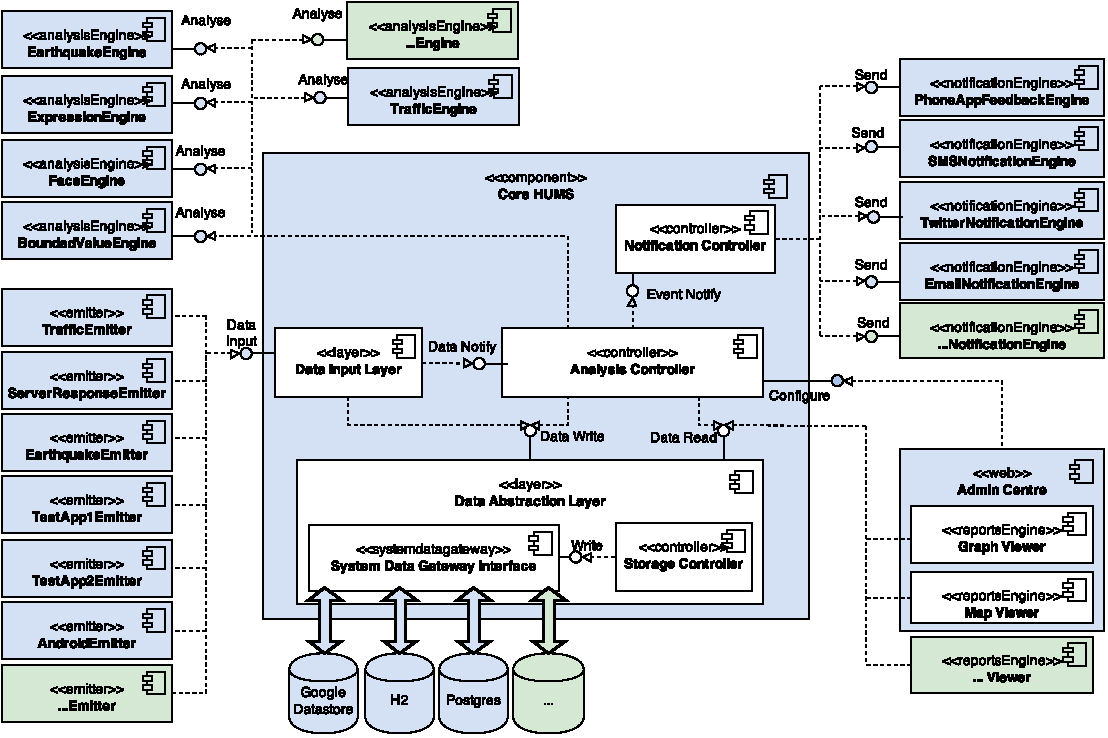
\includegraphics[width=\textwidth]{images/component.pdf}

\subsubsection{Component and Connector View}
\hl{TODO Rosy}

% Put in figure
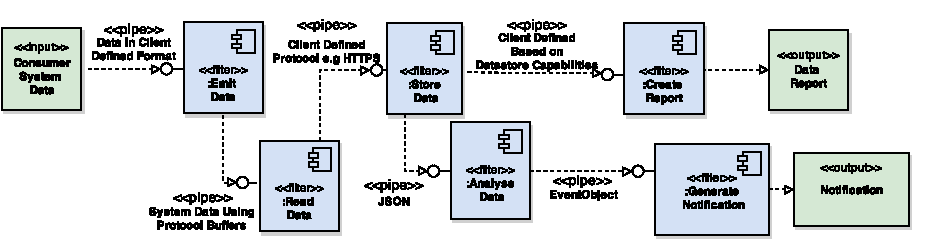
\includegraphics[width=\textwidth]{images/pipesAndFilters.pdf}

\subsubsection{Behavioural View}
\hl{TODO Andy}

\subsubsection{Deployment View}
\hl{TODO Joe}
%-------------------------------------------------------------%
%-------------------DEVELOPMENT-------------------%
%-------------------------------------------------------------%
%   Notes: 					         	 %
%  	- Reference risks constantly, lots and lots	 %
%	- Reference requirements and scenarios 	 %
%-------------------------------------------------------------%
\section{Development}
\label{sec:dev}
\hl{TODO Prehaps Intro}

\subsection{Interim Implementation Summary}
\label{sec:interim_summary}
\hl{TODO ADAM}

\subsection{Changes Since the Interim Report}
\label{sec:changes}
\hl{TODO All}

\subsection{Core Development}
\label{sec:core}
\hl{Andy/Rosy: Config files, gui, server shiz}

A lightweight Jetty server was also added to the core so that the Admin Centre can be served from the same system that the Core runs on. This enables further integration between the configuration files and the web interface created for easily administering them, and avoids any custom server having to be manually set up by the Consumer by automating the process.

\subsection{Monitoring}
\label{sec:monitor}
In this section we describe what data our HUMS currently monitors. We created six sample Data Emitters for this stage of the project, in order to demonstrate the tailorability of our HUMS. These show how the HUMS can integrate with existing applications, and APIs, as well as how it can be used with specially made applications. An end user would be able to quickly create a Data Emitter for their own application by using the interfaces provided with our HUMS.

\subsubsection{Test Applications} \label{subsec:tapp}
\hl{TODO Michael/Ant}

Part of our task was monitoring the provided test applications, treating them as black-box systems we knew nothing about. For the first we simply monitored the memory and CPU usage, but for the second we also added state, number of threads, last processor it was run on, and working directory. For this we created a process monitoring engine which is capable of tracking information from a process.

The monitoring engine utilises the System Information Gatherer (SIGAR) API. SIGAR is a cross-platform API which allows system information and process information to be read, without worrying about which implementation for reading that information the platform provides. The information gathered by this engine is forwarded to the core for analysis.

\subsubsection{Earthquakes and Traffic}
In order to ensure our HUMS is capable of receiving, analysing, and reporting data through various external APIs, we updated our earthquake Data Emitter and added an additional traffic Data Emitter, monitoring real time UK traffic accidents and incidents. The earthquake data is in a JSON format and the traffic data is in an XML format, which are both standard and commonly used data formats. These two emitters demonstrate the extensiblility of the HUMS as similar additional Data Emitters can easily be created to read data from other sources, which would likely also use XML or JSON formats.

\subsubsection{Server Responsiveness}
A common use of existing HUMS systems is in monitoring the responsiveness of websites and servers, alerting users and staff if the system becomes unavailable. In order to ensure our HUMS was capable of such a task, we implemented a response time data emitter which determines the response time of requests to a given website \footnote{thalesgroup.com} and sends this data to the core for analysis.

\subsubsection{Android Mobile Application}
\hl{TODO Finish Tom}

To explore the possibilities surrounding monitoring remote systems over network communication, we created an Android application, with three test systems allowing us to demonstrate that our HUMS is capable of this. Screenshots of the Android application are shown in Figure~\ref{fig:android}.

The first system simulates a car monitoring system,allowing users to select values for a number of sensors and then push them to the core remotely. In the real system the user would not set the values or manually push them as it would all be automatic, however, for the purposes of demonstrating the functionality we choose to manually update the data.

The second system is a phone battery monitoring system, which allows the user to define how long they would like to use their mobile device for and based on the given battery life, uses the HUMS to determine which services can stay on in order for this target to be met, the HUMS then feeds back into this system, toggling those services. This system was designed to show how our HUMS is capable of monitoring a system, and feeding information back to alter the systems behaviour.

The final system performs face recognition, collecting face data using the built-in camera, forwarding that data to the core for analysis and notification, if appropriate. This system was included to show how our HUMS allows for fast, complex, and specific data analysis, in this case using computer vision algorithms.

\begin{figure}[h]
\centering
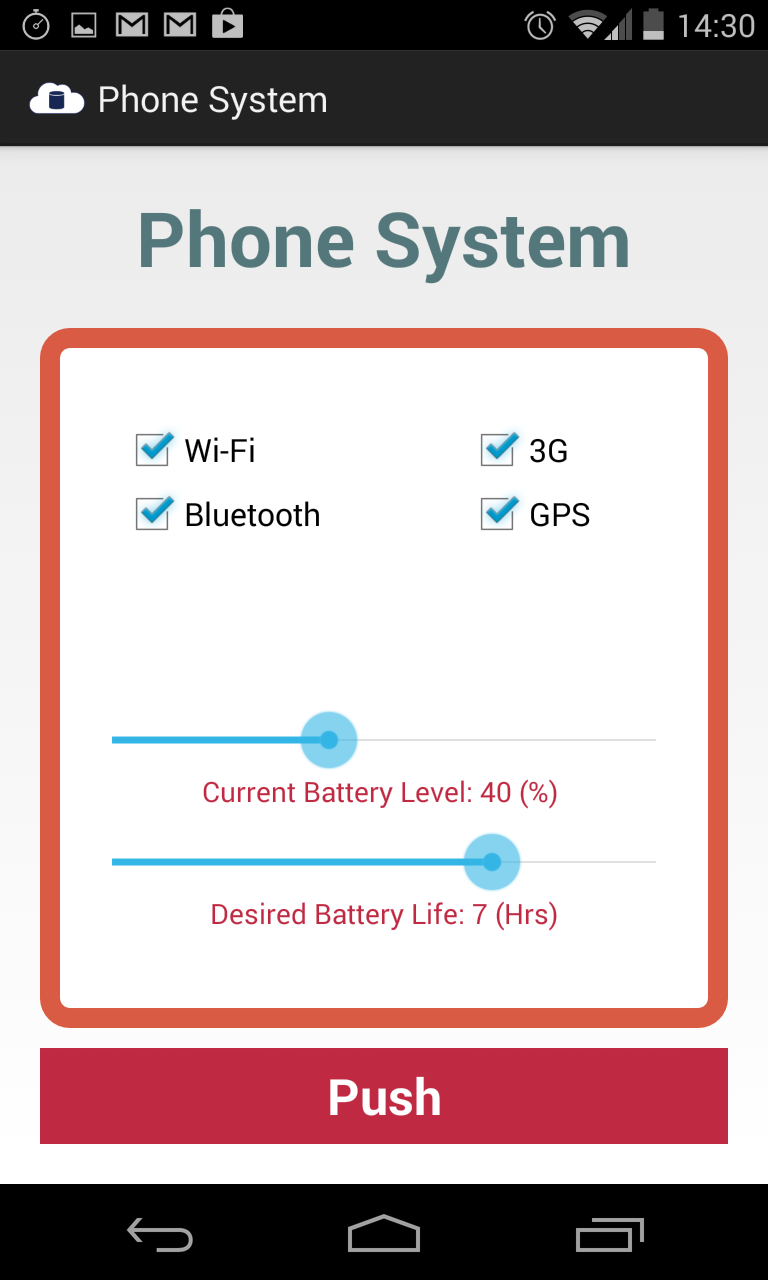
\includegraphics[width=4.3cm]{images/phoneApp.png}
\hspace{0.5cm}
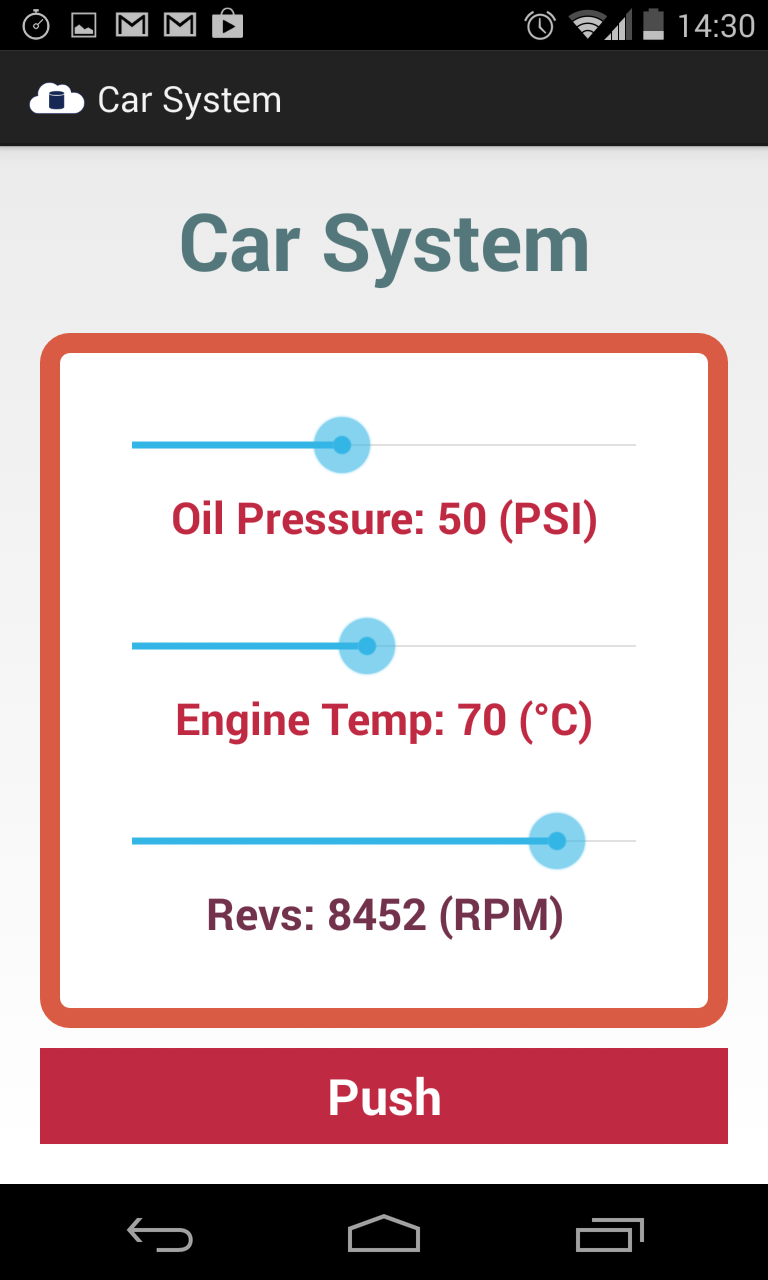
\includegraphics[width=4.3cm]{images/carApp.png}
\hspace{0.5cm}
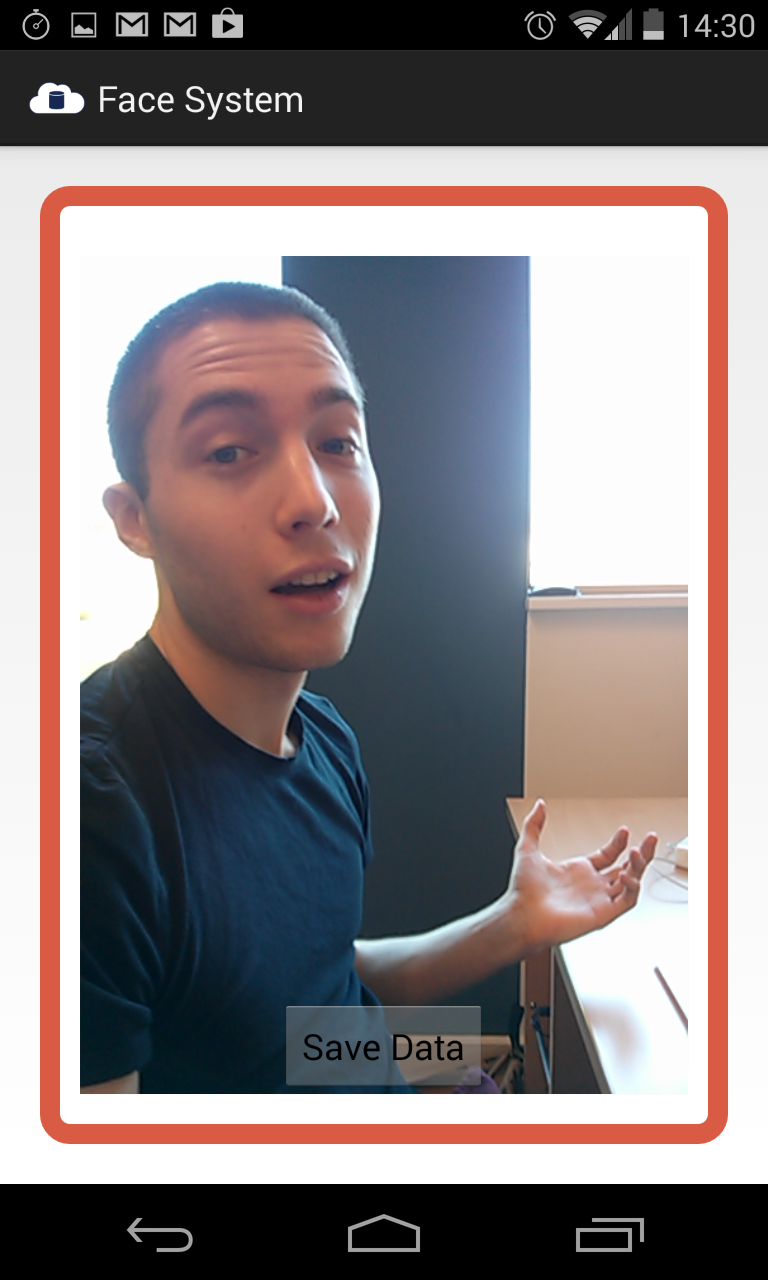
\includegraphics[width=4.3cm]{images/faceApp.png}
\label{fig:android}
\caption{\hl{TODO}}
\end{figure}

\subsection{Data Analysis}
\label{sec:analysis}
\hl{TODO INTRO Joe/Andy/Rosy}

\subsubsection{Generic Bounded Sensor Value Engine}
\hl{TODO A Team -- this is the new and improved mean engine}

\subsubsection{Generic Expression Engine}
\hl{TODO Tom}
%%with a default behaviour of sending an email notification if a request takes more than 5 seconds. ---- server app

To allow for sensors which provide a combination of numeric and string data to use the expression engine, it interprets only the data which is necessary.

\subsubsection{Phone Analysis Engine}
\hl{TODO Rosy}

\subsubsection{Face Analysis Engine}

\hl{TODO Tom/Joe Face Recognition for Security}
% TODO Separate analysis from sensing
The Android app collects face data, forwarding it to the Core for analysis, where notifications are generated, notionally granting or denying access to a secure system. This module shows off the ability of sensors and analysis engines to work together to perform complex tasks, which can be tailored using the Core configuration file.

The face recognition process is two fold: An image is captured and its dimensionality is reduced by the Android app before being sent on to the Core, then the \texttt{FaceAnalysisEngine} takes this face description and analyses it to decide if the face is authorised or not.

The face description in the Android app is computed using the Local Binary Patterns Histogram (LBPH) \cite{ahonen2006face} method. Each pixel in the image is reduced to a bit-vector describing whether each of the neighbouring pixels is brighter or darker than it (although what constitutes a neighbour can be varied to control for scaling). These bit-vectors are then used to generate a histogram. All \emph{uniform bit patterns}, those which have at least two $1$s in a row and no more than two transitions between runs of $1$s and $0$s, have a separate bin and all other patterns have a single bin. A histogram is made for each of a fixed number of regions in the image to ensure that some degree of locality is kept. Each histogram is then concatenated to create the full description vector---the \emph{spatially enhanced histogram}. This results in a compressed description of the image which attempts to preserve the information content pertaining to face description. This is the data which is then transmitted to the Core.

When the histogram data is received by the \texttt{FaceAnalysisEngine}, it is compared against the example authorised faces using the Chi-Squared distance measure, authorising the face provided by the sensor if its distance from any of the example faces provided by the configuration file is less than some threshold, also given by the configuration file.

% TODO This method is robust to lighting and pose \cite{ahonen2006face}

\subsubsection{Other Analysis Engines}
\hl{TODO Ant}
The analysis system is expansible. Hence, it is easy to add further analysis engines to the system. This can easily be done by extending the AnalysisEngine base class, and implementing the required methods. 

\subsection{Data Storage}
\label{sec:store}
\hl{TODO INTRO: Joe||Andy||Rosy}

% %This to be split across the sections below
To improve the tailorability of the system and address risks \emph{R.6} and \emph{R.7}, three different datastores are supported. Two remote data sources, Google app engine and a Postgres instance hosted on Heroku or a local H2 instance. Clients can change between datastores with ease by updating their configuration file.

\hl{Google app engine connection stuff is nonsense, uses TCP}

Both Google App Engine and Heroku are Platform as a Service solutions, they both provide a remote datastore to the HUMS. Communication between a clients HUMS and the remote datastore takes place over HTTP. Both Heroku and App Engine provide a guaranteed uptime of $99.99\%$, as such the reliability and speed of the connection to the remote datastore will be largely influenced by a clients internet connection.

For real-time applications that require high performance and low response times a local H2 instance is offered. H2 is a Java library that implements a simple, self-contained, serverless, transactional SQL database. H2 can be run in embedded or server mode, its small storage footprint of $1.5$MB and low memory usage make it ideal for use in resource constrained environments. 

Connection pooling was used for all datastores. The process of opening, maintaining and deleting connections is resource intensive and a performance bottleneck. A connection pool provides a cache of reusable database connections, connections only need to be created once and shared between components that require data access. The HikariCP Java library was used to simplify the implementation of database connection pools. 

Prepared statements were used across all datastore. They are compiled once and then reused many times leading to significant gains in performance. Finally, prepared statements offer improved security with SQL injection attacks rendered useless with all user input being treated as data and thus not altering the characteristics of data queries.

\subsubsection{Google App Engine Storage}
\hl{TODO Adam/Rosy}

\subsubsection{H2 Storage}
\hl{TODO Adam}

\subsubsection{Heroku Storage}
\hl{TODO Adam}

\subsection{Data Reporting and Event Notifying}
\label{sec:report}
\hl{INTRO: Rosy||Joe||Andy}

\subsubsection{SMS Notifications}
A notification engine was created than can send SMS text messages to mobile phones. This is useful functionality for a HUMS due to the near ubiquitousness of mobile phones in modern life; a User is likely to have their phone with them most of the time so can instantly be notified and informed of anything the HUMS needs to flag up, and then react appropriately. It is a quick and efficient notification method and one that works across all phone platforms. To build this engine we utilised the service offered by the communications company Twilio, who have a large infrastructure for telecommunications and offer an easy to use API.

\subsubsection{Email Notifications}
The email notification example engine provided is similar in functionality to that in the interim report. It can be configured to send email notifications for events to any email address, and may be useful for more detailed or more frequent notifications.

\subsubsection{Twitter Notifications}
\hl{TODO Rosy}

\subsubsection{Android Application Feedback Notifications}
\hl{TODO Rosy}

\subsubsection{Map Report}
The map reporting engine created in the interim report was improved on, making it into a more generic reporting engine that can be used with any latitude and longitude data. This is demonstrated through its use with both the earthquake and the traffic data. Map reports are generated on demand by the User through the Admin Centre, and can then automatically update with the latest data that is input to the HUMS to provide live information.

\subsubsection{Graph Report}
Similarly to the map reporting engine, the graph reporting engine has been enhanced since the interim report and is now a separate engine that can be used to graph different data. The data from both test applications is graphed in the Admin Centre using this engine, showing its flexibility of use. The graph reports generated can also automatically update to show live data.

\subsection{Admin Centre}
\label{sec:admin}

The prototype Admin Centre previously created has been updated and refined to provide a central locations for the User to control the operation and settings of the HUMS. By offering this through a web interface it provides a more familiar and user friendly way for the configuration to be viewed and edited without having to manually edit configuration files. It also means that the Admin Centre can be accessed remotely from a number of different devices and not just from where the core is being run.

The Admin Centre also provides the reporting facilities of the HUMS, with two example reporting engines currently created. A graph report is available and can be used with data like that from the first and second test applications, and a map report is available which is more applicable to data from the earthquake or traffic monitoring.

The updates to the Admin Centre have developed the previous prototype into a fully functioning system that integrates with the HUMS and presents real data and options to the User that they can interact with and update to have effect on the running HUMS instance.

\begin{figure}[b!]
    \begin{subfigure}{0.49\textwidth}
        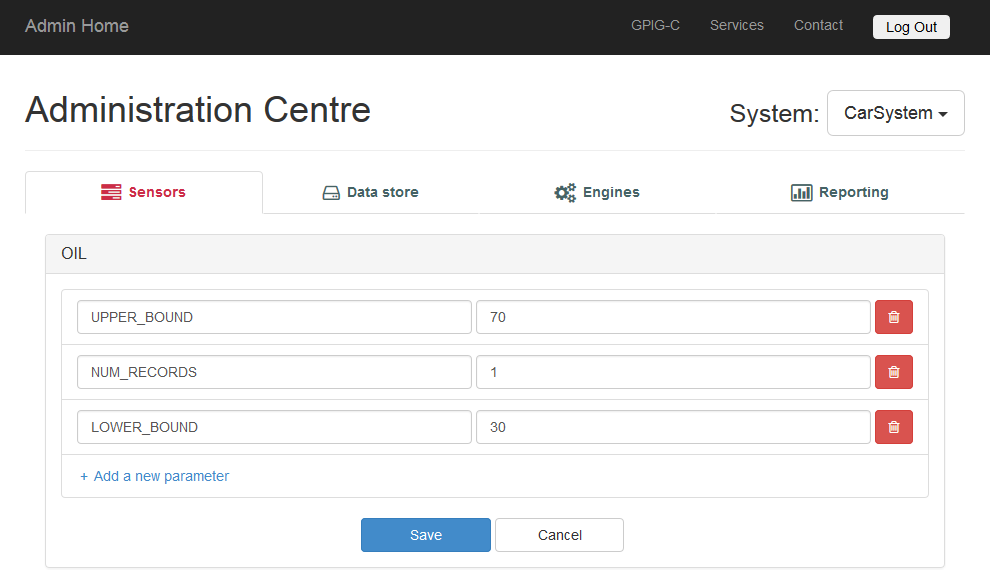
\includegraphics[width=\textwidth]{images/admin-centre_sensors}
        \caption{Sensors}
        \label{fig:admin-centre_sensors}
    \end{subfigure}
    ~
    \begin{subfigure}{0.49\textwidth}
        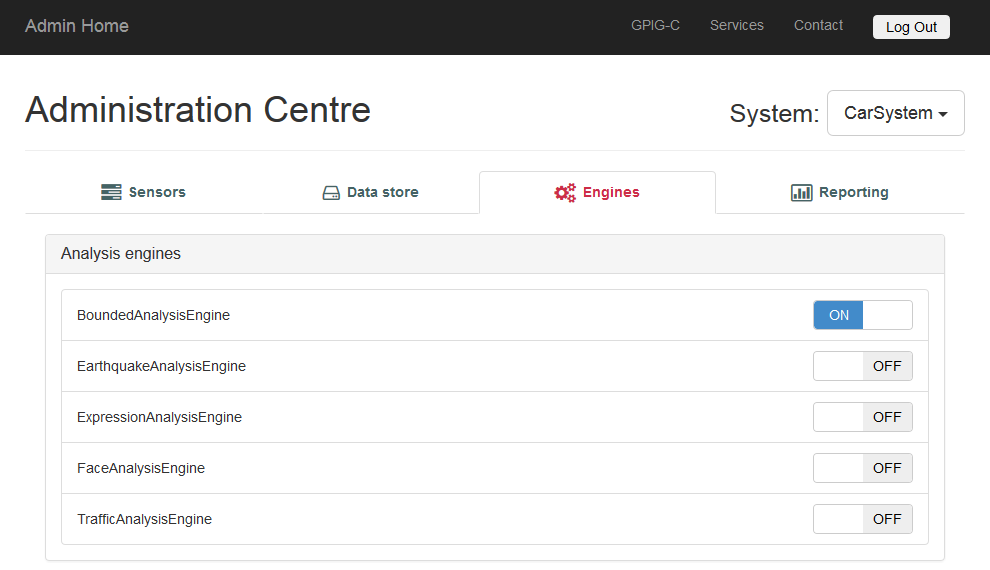
\includegraphics[width=\textwidth]{images/admin-centre_engines}
        \caption{Engine}
        \label{fig:admin-centre_engines}
    \end{subfigure}
	\vspace{0.2cm}

    \begin{subfigure}{0.49\textwidth}
        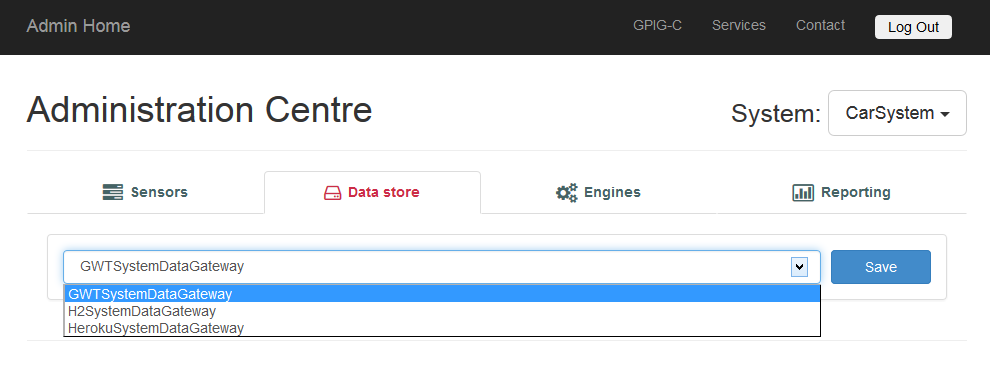
\includegraphics[width=\textwidth]{images/admin-centre_data}
        \caption{Data store}
        \label{fig:admin-centre_data}
    \end{subfigure}
	~
	\begin{subfigure}{0.49\textwidth}
        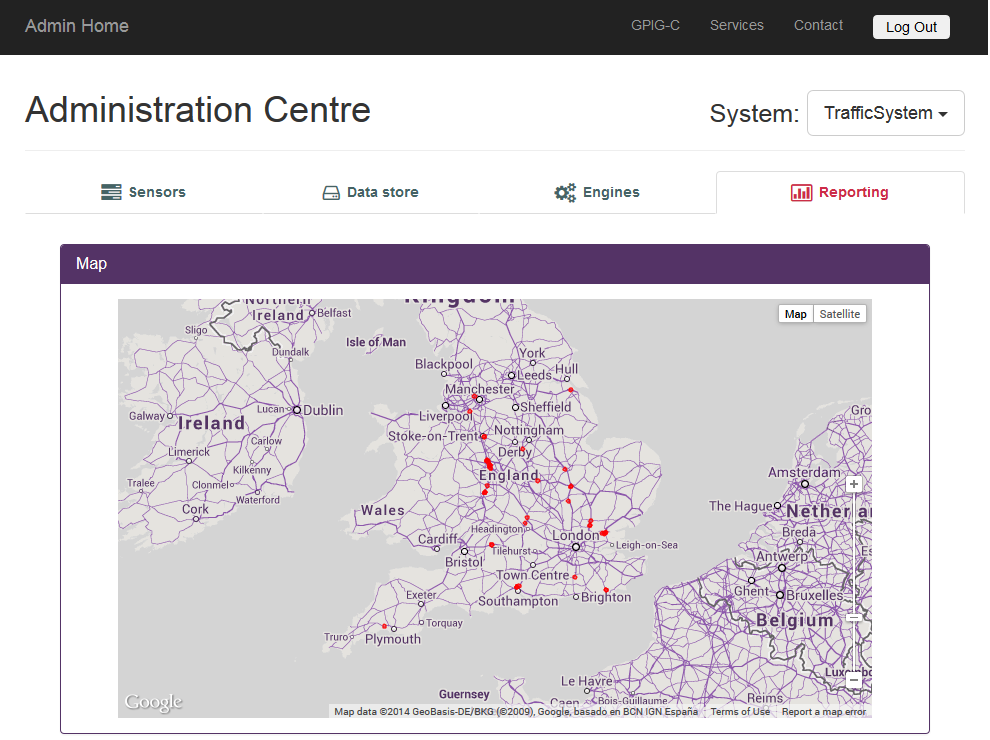
\includegraphics[width=\textwidth]{images/admin-centre_report}
        \caption{Reporting}
        \label{fig:admin-centre_report}
    \end{subfigure}
    \caption{Screenshots of the Admin Centre}
	\label{fig:admin-centre}
\end{figure}

%-------------------------------------------------------------%
%-----------------------PROTOTYPE-----------------------%
%-------------------------------------------------------------%
\section{Prototype Implementation Evaluation}
\label{sec:prototype}
\hl{INTRO: Rosy||Joe||Andy}

\subsection{Evaluation Against Requirements, Qualities, and Scenarios}
\label{sec:req_eval}
\hl{TODO Ant}

\subsection{Evaluation on Test Application 1}
\label{sec:test_app1}

We decided to monitor the memory and CPU usage of the test application, and our initial implementation simply queried the operating system for these values, using the Sigar library. However, this did not work as the JVM manages its own heap internally. We then changed to directly querying the target JVM for its memory usage using the JMX libraries, which was successful.

By using these cross-platform and established libraries, our monitor can be generalised to more than just the test application. This is illustrated by how easily we were able to reuse it as the basis of the second test application.

\subsection{Evaluation on Test Application 2}
\label{sec:test_app2}

Using iotop under Ubuntu 14.04, we were able to verify that the test application did not perform any notable IO operations. Using Wireshark under the same system, no network activity was detected either.

We decided to monitor the process memory usage, CPU usage, state (idle, running, sleeping, stopped, or zombie), working directory, number of threads, and which processor it was last run on. We were able to base the monitor on that developed for the first test application with only minor changes. We decided to monitor the threads because none of the other metrics produced an interesting result, however we found that only one thread was used.

\subsection{Evaluation of the HUMS SaaS}
\label{sec:hums_saas}
\hl{TODO Andy}
% also mention PaaS here?


\subsection{Evaluation of Additional Engines}
\label{sec:additional}
\hl{TODO Rosy\&Tom\&Adam}

%-------------------------------------------------------------%
%---------------------COMMUNICATION-------------------%
%-------------------------------------------------------------%
\section{Customer Communication \hl{Someone.... please not me}}
\label{sec:customer_comms}

%-------------------------------------------------------------%
%----------------------CONCLUSION----------------------%
%-------------------------------------------------------------%
\section{Conclusion}
\label{sec:conclusion}
\hl{TODO All}

\subsection{Summary}
\label{sec:summary}
\hl{TODO All}

\subsection{Reflection}
\label{sec:reflection}
\hl{TODO All}

\bibliography{report-refs}
\bibliographystyle{IEEEtran}
\end{document}
}
